%%=================================================%%
%%						TITRE DU DOCUMENT (1 PAGE)
%							  Pas totalement fini
%%=================================================%%

\begin{titlepage}
\begin{center}

% Upper part of the page. The '~' is needed because only works if a paragraph has started.


\includegraphics[width=0.60\textwidth]{./page_de_garde/logo_ups.png}~\\[1cm]

\textsc{\LARGE Université Paul Sabatier}\\[1.5cm]

\textsc{\Large \bf Conception et mise en \oe uvre de commande à temps réel\\[0.5cm]}

% Title
\HRule \\[0.4cm]

{\huge \bfseries  - Rapport 1 : \textsc{Analyse théorique} -}

\HRule \\[1.5cm]

% Author and supervisor
\begin{minipage}{0.4\textwidth}
\begin{flushleft} \large
\emph{Auteurs:}\\
Lucien \textsc{RAKOTOMALALA}\\
David \textsc{TOCAVEN}\\
\end{flushleft}
\end{minipage}
\begin{minipage}{0.58\textwidth}
\begin{flushright} \large
\emph{Encadrants:} \\
\textbf{ Sylvain \textsc{Durola}}\\
\textbf{ Frédéric \textsc{Gouaisbaut}}\\
\textbf{ Yann \textsc{Labit}}
\end{flushright}
\end{minipage}
\newline
\newline

% une éventuelle image
%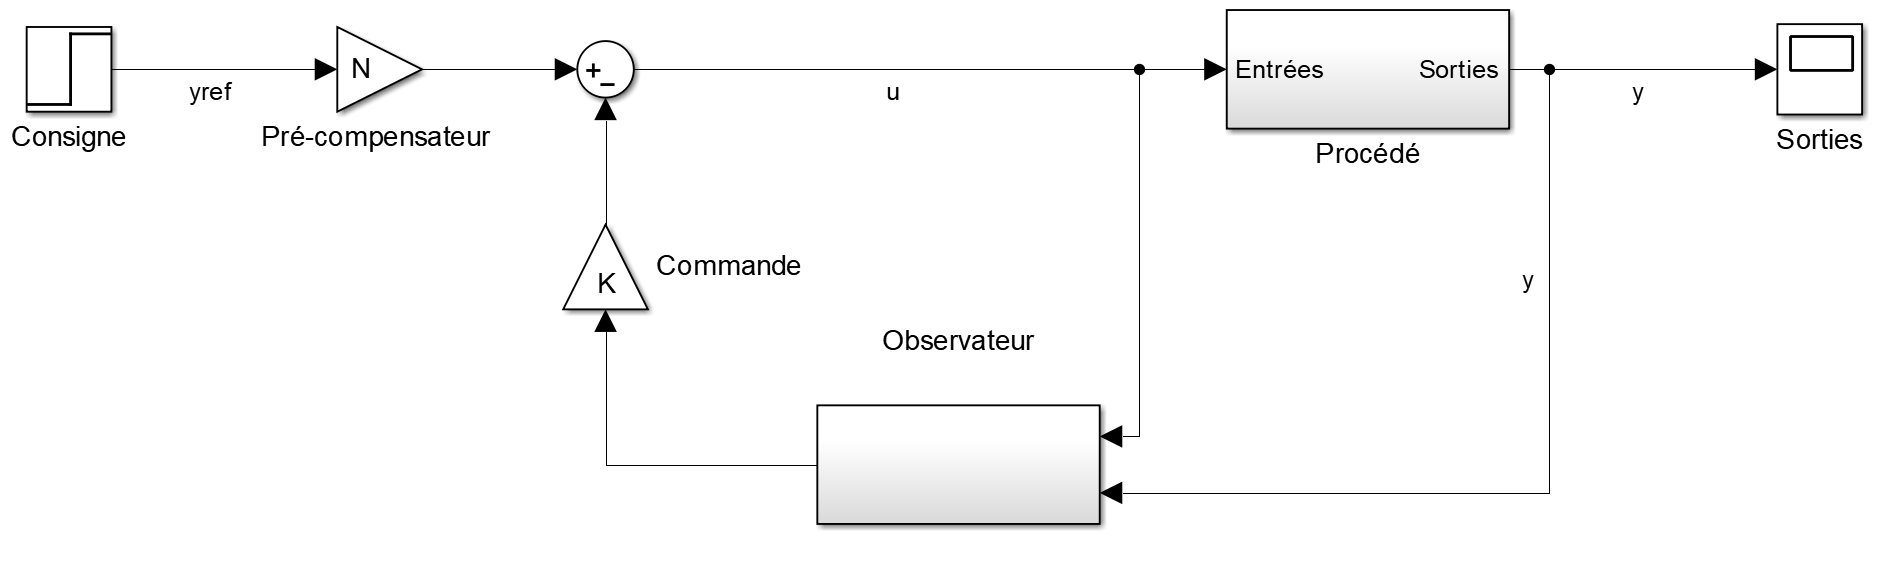
\includegraphics[width=.6\textwidth]{./page_de_garde/schemaRE.png}~\\[1cm]

\vfill
% logo fsi & eea
\begin{tabular}{cc}
   
\includegraphics[height=2cm]{./page_de_garde/logo_fsi.png} \hspace{2cm} &
    \hspace{2cm}
   
\includegraphics[height=2cm]{./page_de_garde/logo_eea.jpg} \\
\end{tabular}

% Bottom of the page
{\large \today}

\end{center}
\end{titlepage}
